\documentclass[12pt,a4paper,titlepage]{report}
\usepackage[utf8]{inputenc}     % accents dans la source
\usepackage[T1]{fontenc}        % nouvelle norme latex
\usepackage[normalem]{ulem}     % 
\usepackage[french]{babel}      % supporter le français
\usepackage{verbatim}           % coder en VERBATIM
\usepackage[pdftex]{graphicx, color}
\graphicspath{{figs/}}
\DeclareGraphicsExtensions{.jpg,.png}
\usepackage{url}                %
\usepackage{hyperref}           % utiliser les liens hypertextes
\usepackage{color}              % utiliser les couleur 
\usepackage{pifont}             % des symboles et des figures
\usepackage{fancybox}           % carrés 
\usepackage[a4paper,rmargin=2cm,lmargin=2cm,tmargin=2cm,bmargin=2cm]{geometry}  % mise en page 
\usepackage{listings}           % du code dans latex
\usepackage{fancyhdr}
\usepackage{float}


\begin{document}
\begin{titlepage}
  \begin{flushleft}
    \vspace{3mm}
    
\includegraphics[width=3cm]{upmclogo_m.png}\\
  \end{flushleft}
  \vfil
  \vfil
  \begin{center}
    \Huge\textbf{{PPAR}}\\
    \hrulefill\\
    \Huge\textit{{Probleme des N-CORPS}}\\
  \end{center}
  \hrulefill\\
  \vfil
  \noindent \textbf{ALAHYANE} \bsc{Rachid}
  \hfill 
  \href{mailto:rachid.alahyane@etu.upmc.fr}{rachid.alahyane@etu.upmc.fr}\\ 
  \textbf{CASTELLANOS} \bsc{Cuauhtemoc}
  \hfill 
  \href{mailto:cuauhtemoc.castellanos@etu.upmc.fr}{cuauhtemoc.castellanos@etu.upmc.fr}\\
  \vfil
  \begin{center}	
    \shadowbox{\footnotesize{\emph{PPAR 2009 - \today}}}
  \end{center}
\end{titlepage}





%\tableofcontents
\lhead{PSIA 2009}
\rhead{Peersim}
\renewcommand\headrulewidth{2pt}


\section*{Objectifs}
\thispagestyle{fancy}
\par L'objectif de ce projet consiste à faire une simulation de la propagation de la grippe A dans une population avec des contraintes bien définies. 
\par Dans un premier temps, la simulation portera sur une population où les habitants sont voisins dans un sens et pas nécessairement dans l'autre, représentée par un graphe orienté. Les habitants peuvent être vaccinés ou pas. 
\par Dans la deuxième partie, les liens sociaux entres les habitants seront présentés d'une manière plus réaliste. Dans notre alogorithme, ces liens seront représentés par un graphe non orienté.

%%%%%%%%%%%%%%%%%%%%%%%%%%%%%%%%%%%%%%%
% PREMIERE PARTIE
%%%%%%%%%%%%%%%%%%%%%%%%%%%%%%%%%%%%%%%

%%%%%%%%%%%%%%%%%%%%%%%%%%%%%%%%%%%%%%%
% PREMIERE PARTIE
%%%%%%%%%%%%%%%%%%%%%%%%%%%%%%%%%%%%%%%

\section*{Première partie}
\subsection*{Population avant vaccination}
Après avoir lancé la simulation avec une population non vaccinée, nous avons obtenu 
les résultats représentés par les figures \ref{fig:1-1-nb-malades} et \ref{fig:1-1-nb-morts}   

\begin{figure}[htbp] 
%\begin{figure}[h]
  \centering
  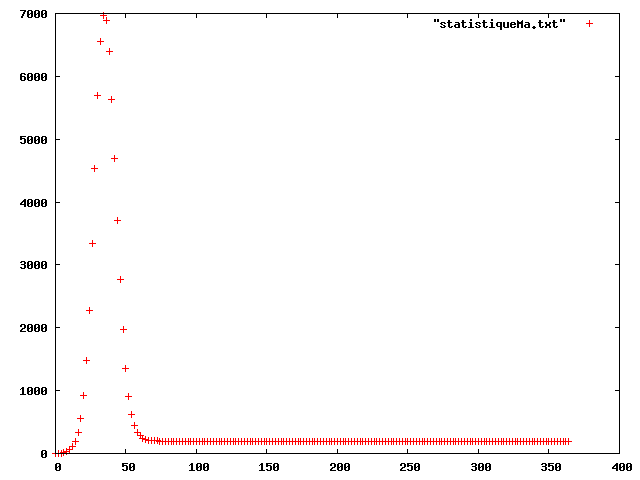
\includegraphics[width=15cm]{1-1-statistiqueMa.png}
  % usecase.png: 985x829 pixel, 72dpi, 34.75x29.25 cm, bb=0 0 985 829
  \caption{Nombre de personnes contaminées par jour}
  \label{fig:1-1-nb-malades}
\end{figure}

\begin{figure}[htbp] 
%\begin{figure}[h]
  \centering
  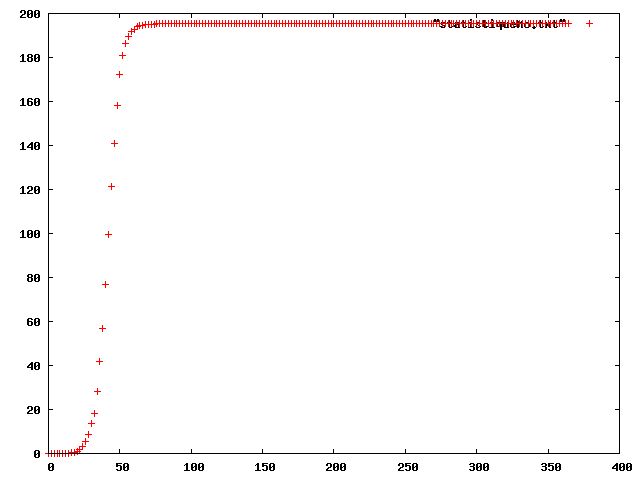
\includegraphics[width=15cm]{1-1-statistiqueMo.png}
  % usecase.png: 985x829 pixel, 72dpi, 34.75x29.25 cm, bb=0 0 985 829
  \caption{Nombre de personnes mortes par jour}
  \label{fig:1-1-nb-morts}
\end{figure}

\subsection*{Population après vaccination}
Dans cette partie, nous avons lancé plusieurs simulations sur des populations dans 
lesquelles  le taux de vaccination valait entre 0\% et 100\%. Les figures  \ref{fig:1-2-nb-malades} 
et \ref{fig:1-2-nb-morts} représentent les résultas obtenus.

\begin{figure}[htbp] 
%\begin{figure}[h]
  \centering
  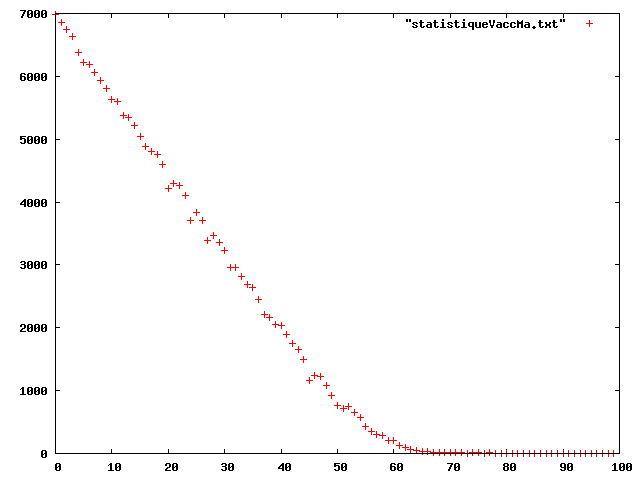
\includegraphics[width=15cm]{1-2-statistiqueMa.png}
  % usecase.png: 985x829 pixel, 72dpi, 34.75x29.25 cm, bb=0 0 985 829
  \caption{Taux de contamination maximal en fonction du pourcentage de population vaccinée}
  \label{fig:1-2-nb-malades}
\end{figure}

 \begin{figure}[h]
  \centering
  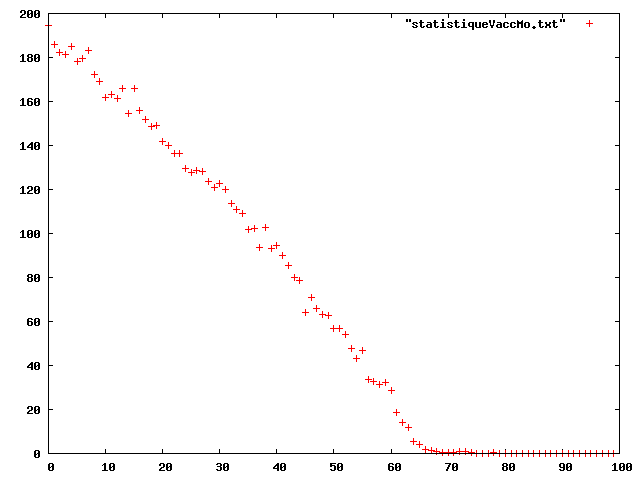
\includegraphics[width=15cm]{1-2-statistiqueMo.png}
  % usecase.png: 985x829 pixel, 72dpi, 34.75x29.25 cm, bb=0 0 985 829
  \caption{Taux de mortalité maximal en fonction du pourcentage de population vaccinée}
  \label{fig:1-2-nb-morts}
\end{figure}


%%%%%%%%%%%%%%%%%%%%%%%%%%%%%%%%%%%%%%%
% DEUXIEME PARTIE
%%%%%%%%%%%%%%%%%%%%%%%%%%%%%%%%%%%%%%%

%%%%%%%%%%%%%%%%%%%%%%%%%%%%%%%%%%%%%%%%
% DEUXIEME PARTIE
%%%%%%%%%%%%%%%%%%%%%%%%%%%%%%%%%%%%%%%

\section*{Deuxième partie}
Dans cette partie, les liens sociaux sont représentés de manière très réaliste. Un lien de 
connaissance entre individus de la ville est bidirectionnel.  
\subsection*{Population avant vaccination}
Les figures \ref{fig:2-1-nb-malades} et \ref{fig:2-1-nb-morts} représentent les résultats obtenus:
\begin{figure}[h]
  \centering
%  \includegraphics[width=15cm]{diagrams/pnml-web-usecase.png}
  % usecase.png: 985x829 pixel, 72dpi, 34.75x29.25 cm, bb=0 0 985 829
  \caption{Nombre de personnes contaminées par jour}
  \label{fig:2-1-nb-malades}
\end{figure}

\begin{figure}[h]
  \centering
%  \includegraphics[width=15cm]{diagrams/pnml-web-usecase.png}
  % usecase.png: 985x829 pixel, 72dpi, 34.75x29.25 cm, bb=0 0 985 829
  \caption{Nombre de personnes mortes par jour}
  \label{fig:2-1-nb-morts}
\end{figure}

\subsection*{Population après vaccination partielle}
Les figures \ref{fig:2-2-nb-malades} 
et \ref{fig:2-2-nb-morts} représentent les résultas obtenus.
\begin{figure}[h]
  \centering
%  \includegraphics[width=15cm]{diagrams/pnml-web-usecase.png}
  % usecase.png: 985x829 pixel, 72dpi, 34.75x29.25 cm, bb=0 0 985 829
  \caption{Taux de contamination maximal en fonction du pourcentage de population vaccinée}
  \label{fig:2-2-nb-malades}
\end{figure}

 \begin{figure}[h]
  \centering
%  \includegraphics[width=15cm]{diagrams/pnml-web-usecase.png}
  % usecase.png: 985x829 pixel, 72dpi, 34.75x29.25 cm, bb=0 0 985 829
  \caption{Taux de mortalité maximal en fonction du pourcentage de population vaccinée}
  \label{fig:2-2-nb-morts}
\end{figure}



\end{document}
